\documentclass[9pt,twocolumn,twoside]{../../styles/osajnl}
\usepackage{fancyvrb}
\journal{i524} 

\title{Optical Character Recognition}

\author[1]{Saber Sheybani}
\author[1]{Sushmita Sivaprasad}


\affil[1]{School of Informatics and Computing, Bloomington, IN 47408, U.S.A.}


\affil[*]{Corresponding authors: sheybani@umail.iu.edu,sushsiva@umail.iu.edu}

\dates{project-000, \today}

\ociscodes{OCR, Ansible, K-Nearest Neighbor}

% replace this with your url in github/gitlab
\doi{ Report: \url{https://github.com/cloudmesh/sp17-i524/blob/master/project/S17-IR-P012/report/report.pdf}\\
 Code: \url{https://github.com/cloudmesh/cloudmesh.ocr/tree/master/code}}


\begin{abstract}
Optical Character Recognition is a technology for converting images of texts,
into machine encoded text format. In this project, the input data is
in standard image formats and our goal is to recognize the words/letters in the
image as accurately as possible and convert the dataset into TXT
format. The heart of OCR as a pattern recognition system is a classifier.
The images will go through a pre-processing phase which will convert them
into a form that is compatible for feeding to the classifier. Then the classifier
will determine the class of each glyph in the image. The whole recognition system
is installed and operated on the cloud.
\newline
\end{abstract}

\begin{document}

\maketitle

\section{Introduction}

The age of digitalization has made it quintessential to store documents
in a digital form for the purpose of allowing valuable information to
be stored, edited and searchable in the middle of billions of
records. OCR technology is used quite frequently by every industry that
has handwritten, scanned or photographic data.  This project proposal
gives a detailed view on how the OCR technology works, the preprocessing done to remove the noise and the
algorithms used to recognize the images. We have delved deep into some of the basic
concepts used in the implementation process. We have also discussed some
important applications of this technology in the real world and created a benchmark.

\section{Execution Plan}
This execution plan is to show the distribution of work over the time
period of the course.  The steps followed to achieve the final results.
\begin{enumerate}
\item {\bfseries 6 March - 12 March 2017} To implement the OCR, we
  first looked for a dataset to train the algorithm and test it.  The
  desired library to use to write the codes and the complexity of the 
  final goal of the project was discussed.
\item{\bfseries 13 March -19 March 2017}
  Looking for preprocessing steps in order to cleanse noise from the
  image and convert the image into a standard form which makes it adequate
  for later processing.
\item {\bfseries 20 March - 26
    March 2017} Starting to work with Ansible and Cloudmesh Client for running
    tasks on virtual nodes.
\item{\bfseries 27 March- 02 April 2017} starting to deploy individual modules
    for preprocessing, to the virtual machines on Chameleon Cloud service,
    using Ansible. Cloudmesh Client was used to reserve the virtual machines 
    on the cloud services.
\item {\bfseries 03 April- 09
    April 2017} Executing a preliminary form of character recognition using
    K Nearest Neighbour classification and a large dataset.
\item {\bfseries 10 April - 16 April 2017}
    Implementing segmentation of image into lines, words and letters.
\item {\bfseries 17 April - 23 April 2017} Executing benchmark and
  finalizing the project report.
\end{enumerate}

\section{BACKGROUND}
\subsection{OCR Technology}  
 
Optical Character Recognition is a technology which is used to convert
different types of documents that can be in the form of scanned documents,
including handwritten or machine-written into an editable and searchable
form  \cite{www-ocr}. 
The images can be in either the basic black \& white or colored.  The
technology analyzes the structure of the document and divides it
into small refined segments, so that each segment contains one character.
Finally, individual characters are singled out
one by one and fed to a classification algorithm which will return the
closest letter that the individual character could possibly be
identified with.

\section {SYSTEM CONFIGURATION AND TECHNOLOGIES USED}
\subsection{System Configuration}
The python codes and the libraries are run on a Ubuntu 16.04 LTS.

\subsection{Technologies Used}
\begin{enumerate}
  \item {\bfseries Python Programming Language} : An object oriented
  programming language with an open-source license. We chose Python for
  this project as there are many libraries available in Python that
  helps in creating a code for OCR easier. Packages such as PIL,
  Pillow and OpenCV are one of the few libaries that helps in image
  processing.
\item{\bfseries OpenCV } : OpenCV is an open source computer vision
  library.  It is used for building computer vision applications. It
  consists of more than 2500 algorithms including both machine
  learning and computer vision algorithms \cite{opencv-about}. These algorithms are
  devised for facial and image recognition, track any moving objects
  etc. We have used OpenCV 2 for creating a KNN classifier and a few
  of our preprocessing techniques.
  
  \item{\bfseries Ansible} : Ansible is an IT automation tool. It uses
    YAML in order to issue the state of the server
    \cite{www-ocr}. Ansible implements the internal command that is
    required to reach that state which depends on the operating
    system. The ansible playbook which consists of these internal
    commands can be applied to any server or service. There is no
    requirement to instal an additional software on the target system
    as the commands are run over an SSH session.
  \item{\bfseries Cloudmesh Client} : It is an open source client
    interface tool that provides us with an easy-to-use interface for
    accessing cloud services, creating single and multiple VMs, 
    clusters and workstations.We can manage the resources we would
    like to use and customize them as per our requirement to run the
    projects.\\ It provides an interface to execute jobs on High
    Performance Computing clusters \cite{cloudmesh}.The users can use
    just one platform to manage all of the cloud resources. Cloudmesh
    client creates a local copy of the data which results in clouds
    with similar configurations to be created as well.  The default
    features of the Cloudmesh Client allows easy control of the cloud
    as well. Cloudmesh includes an API, commandline client and a
    commandline shell.

\begin{figure}
\centering
\fbox{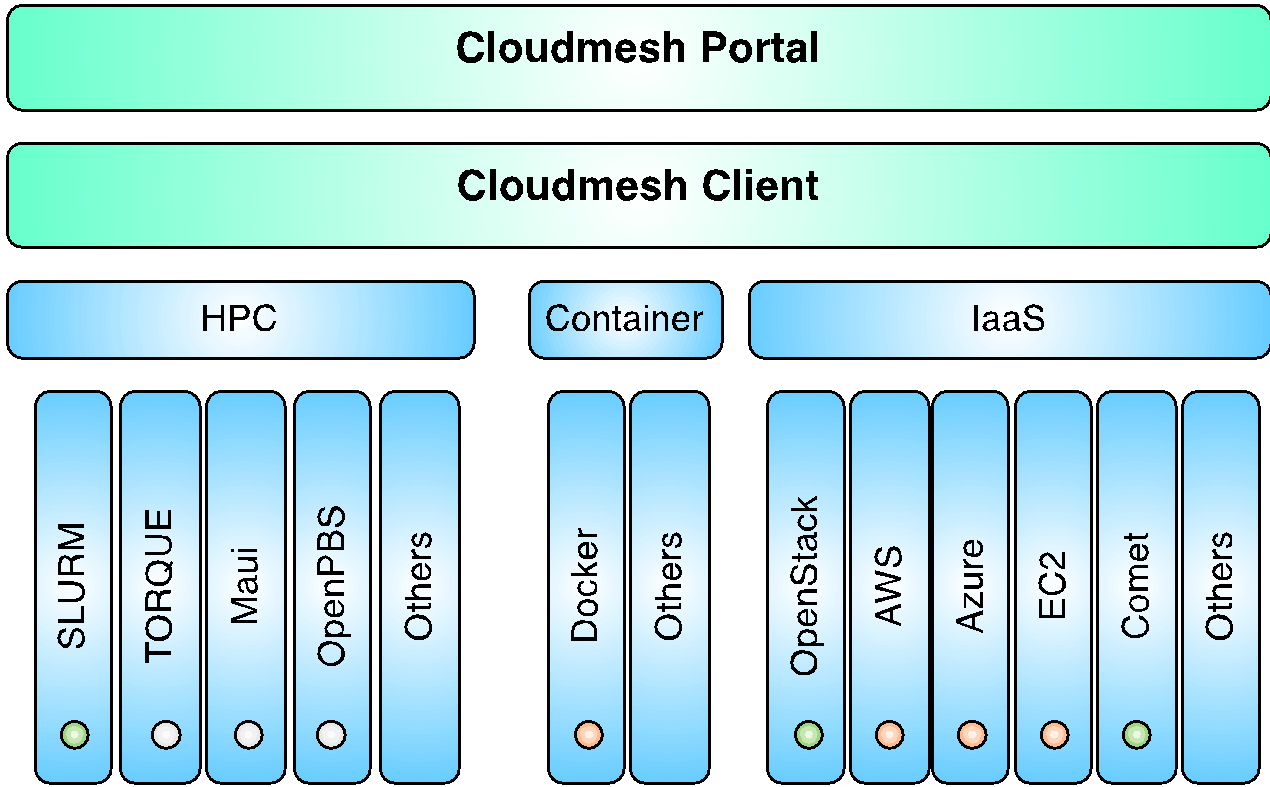
\includegraphics[width=\linewidth]{images/cloudmesh.png}}
\caption{Architecture of Cloudmesh Client \cite{cloudmesh}}
\label{Architecture of Cloudmesh Client}
\end{figure}

\item{\bfseries Chameleon Cloud} :Chameleon cloud provides
  OpenStack Cloud (kilo) using the KVM virtualization
  technology \cite{www-chameleon-openstack}. It is an Infrastructure as
  a Service(IaaS) platform that allows us to create as well as manage
  the virtual environment. The virtual machine that we use here is
  compatible with KVM. Chameleon Cloud also gives access to the
  bare-metal computing resources, which allows administrative rights to
  use cloud for computing experiments \cite{www-chameleon-baremetal}.
\end{enumerate}


\section{Method Survey}

Optical Character Recognition have already been developed in numerous
ways, focusing on different goals. We did a survey on the possible
approaches for character recognition.

The main components of every OCR system can be enumerated as feature
extraction component, and the classifier.

Feature extraction methods can be separated into two groups:
Template matching, and Structural classification \cite{borovikov2014survey}.
In \textbf{Template matching}, the individual pixels of the image
are directly used as features. For each possible character, there is 
one class and one template feature set, associated with it. In classification,
a similarity metric will evaluate the distance of the input character to each
of the templates. And thus, the input will be represented with the class of
the most similar template.

In \textbf{structural classification} structural features of every
character, such as loops and curves, are used as features.

There are various types of classification methods. A number of methods that
have been used for OCR are Nearest-Neighbor, Artificial Neural Networks,
and Support Vector Machines. K-Nearest Neighbor and Artificial Neural Networks
are discussed further as the candidates for our job.

\subsection {K Nearest Neighbour}
It is a non parametric algorithm where each of the training data is considered to have a set of vectors and a class label associated with each vectors. The training set will have the labels for the classes , given the test set it calculates the distance between the training set and the test set and calculate the nearest points. A single value of 'K' is given which allows us to decide how many neighbours influence the classification. Figure \ref{fig:knn} displays a schema of KNN classification.

\begin{figure}
\centering
\fbox{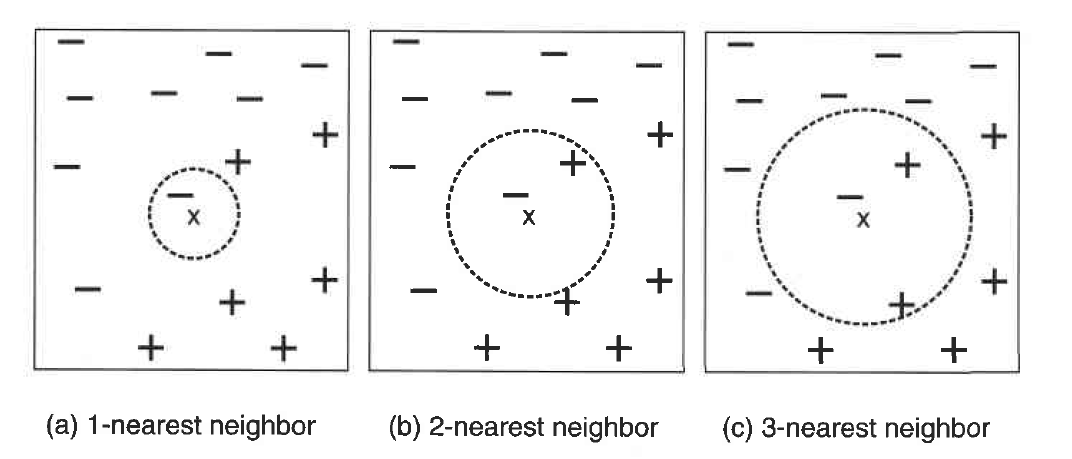
\includegraphics[width=\linewidth]{images/knn.png}}
\caption{Example of k-NN classification \cite{steinbach-book}}
\label{fig:knn}
\end{figure}

\subsection{Feed Forward Neural Networks}
Artificial Neural Network is a paradigm in computing, inspired by the
structure of biological nervous systems. It consists of a network of
processing units, where the output of each unit is a nonlinear
function of its weighted inputs that come from other units. Such
network can be trained to solve different kinds of problems, including
classification and clustering. A feed forward neural networks is one
in which the neurons are organized in a number of layers and each
layer only feeds to the next one, but not to the previous one (no
feedback). However, in a back-propagation process, the errors from one
iteration of classification will be fed back from the output to the
network, in order to modify and improve the network for next
iterations.

Due to simplicity and relatively good performance of KNN, we choose it 
as the classifier for this project. There is an easy to use implementation
of it in OpenCV library.
Our KNN uses euclidean distance as the distance metric to calculate the nearest neighbours for the 'K' value. \\
Euclidean Distance\\$ d(p,q) = \sqrt{ \sigma(p_i - q_i)^2}$\\
For the value of K, 5 is chosen so that it is neither too small and sensitive to the noise nor too large which might result in including the points from other classes.

\section {Preprocessing Techniques}

The steps in an OCR full session are as follows:
Preprocessing: The input images need to be segmented
into units that each of them keep only one glyph (symbol). Also, the
colored or grayscale images will be binarized.  
Feature extraction: The glyphs will be decomposed into features like lines, closed loops,
line direction, and line intersections.  
Character recognition: The
image features will be fed to the classifier and they will be
compared with stored glyph features and the nearest match will be
chosen.

Preprocessing is required on the raw images that we are using to
filter out the required subject and distinguish from any other
unwanted objects from the image such as watermarks, background
subjects etc. We have conducted different preprocessing techniques in
order to remove noise and convert the image into a grey scale format
as color images requires more complex methods of processing

\subsection{ Noise Reduction Techniques}

Noise reduction is done for extracting out any unwanted bit-pattern,
there are linear as well as non-linear techniques for this.  Linear :
In this method is used to remove any isolated pixel noise from the
image. Here the required output filter is taken as a linear
combination of the neighborhood pixels Non- Linear : These kind of
filters are used to replace the value of a particular pixel in order
to remove any kind of impulse noise

\subsection{Histogram Based Method}

It gives a value to the intensity of the pixel and plot it on a
histogram , where darker the image , more the data points would be on
the left and center of the histogram . Lighter the image , more the
data points would be on the right side of the histogram. Using a
histogram equalization method the contrast on the image can be
improved in this case. In the histogram equalization method , an image
is divided into blocks of pixels and an histogram equalization is
done.  This allows us to distinguish the images we actually require
from the other background images . It allows us to enhance the
visibility of the characters’ present on the image.

\subsection{Median Filter}
It is a non-linear noise reduction technique , it is a low pass
filter. In this case the pixel values are taken for an area on the
image and an average of the pixel value is taken and assigned to the
center pixel in that area. Figure \ref{fig:median-schema} displays a schema of
how median filter works. It is an effective means for removing the
salt and pepper noise which are random lines occurring on the image
due to poor quality of the picture or if the image wasn’t scanned
well \cite{medianfilterpreprocessing}. Figure \ref{fig:median} shows the result of
applying a median filter on a scanned image, we can see the reduction
in dots and other marks on the image, making it more smooth and
usable.


\begin{figure}[H]
\centering
\fbox{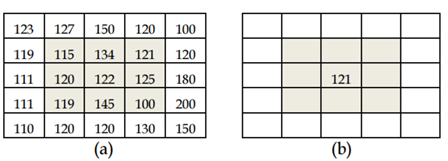
\includegraphics[width=\linewidth]{images/pasted.png}}
\caption{Averaging of a pixel in median filter \cite{medianfilterpreprocessing}}
\label{fig:median-schema}
\end{figure}

\begin{figure}[H]
\centering
\fbox{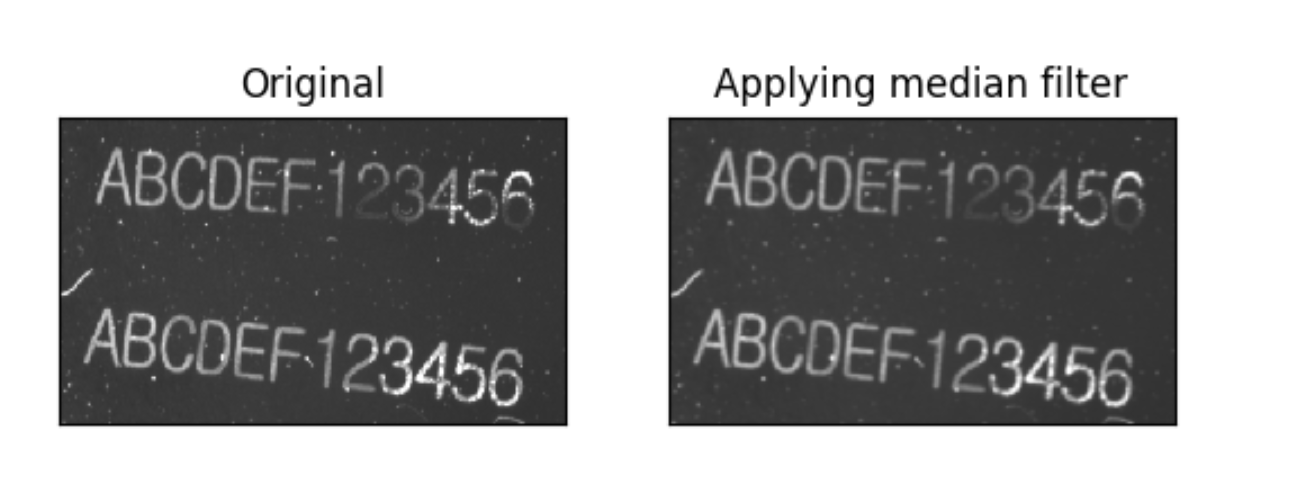
\includegraphics[width=8 cm]{images/medianfilter}}
\caption{Result of applying median filter on a scanned image}
\label{fig:median}
\end{figure}


\subsection{Gaussian Blur}
Gaussian Blur filtwe is a low pass filter which is used to eliminate
isolated pixel noise. Image smoothing is done here using gaussian
filters where the weighted average of the pixel values is computed
with the gaussian coefficients as weight. The filter provides a smooth
texture to the noisy image.

\begin{figure}[H]
\centering
\fbox{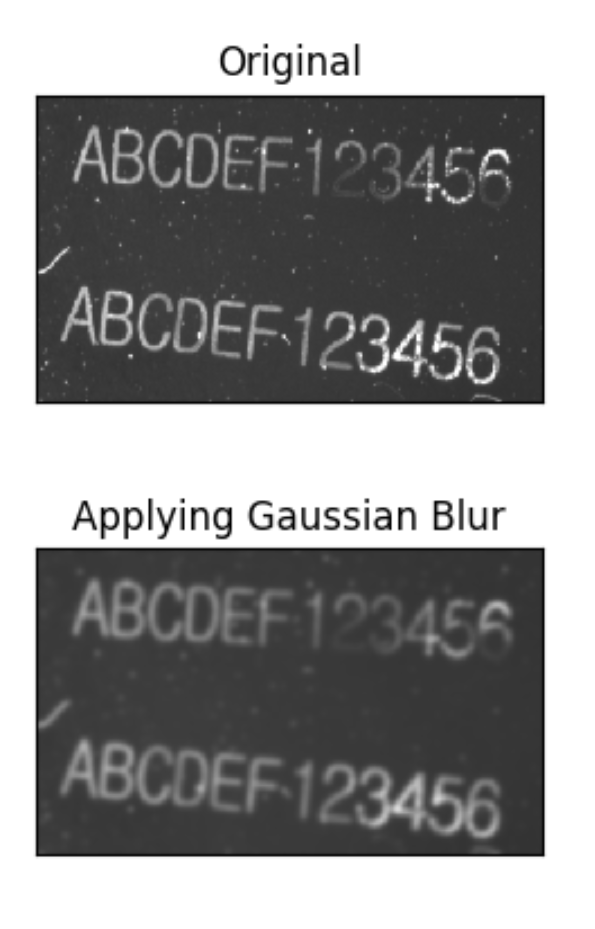
\includegraphics[width=0.25\textwidth]{images/gaussianfilter.png}}
\caption{After applying gaussian filter on the image preproccesed with median filter}
\end{figure}


\subsection{ Binarization}

Otsu’s method \cite{otsu1975threshold}: Otsu’s method concludes finding
the best intensity threshold to separate two classes, often background
vs foreground but not always. The algorithm tries to find a separation
point that has the minimum weighted within class variance.  If the
input images are grayscale, the algorithm will simply find a threshold
that any intensity below that will be considered as the background and
the intensity of the corresponding pixels will be rounded to
zero. Similarly, the intensities above the threshold will be rounded
to 1. The resulting image (array) will be binary.

\begin{figure}[H]
\centering
\fbox{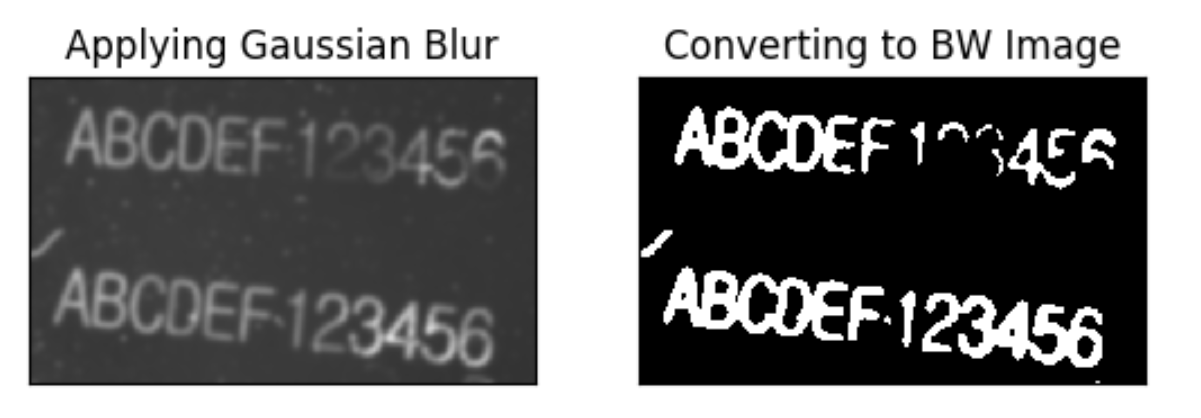
\includegraphics[width=8 cm]{images/binarization.png}}
\caption{Applying binarization after applying gaussian filter}
\end{figure}

\subsection{ Segmentation}
Segmentaion of the image happens in multiple levels, namely lines, words 
and letters. Application of all of these three will enable the conversion
of whole pages of scanned documents into text format.
In this project, segmentation at all levels is implemented using 
projection profile approach. Projection of the intensities on the vertical
axis will differentiate the rows that contain some text, from the ones that
only include the background.
\newline
For word segmentation if the number of background columns are more than a 
threshold, the two letters will be considered as incorporating different words.
The background columns are detected using projection on the horizontal axis, but only
for the rows that are included in the current line. Thresholds are defined using
expert views in typography \cite{dowding1995finer}.
\newline
The letter segmentation is simply done after one background column is found.
The figure \ref{fig:segment} displays the application of our segmentation algorithm
on a sample image.

\begin{figure}[H]
\centering
\fbox{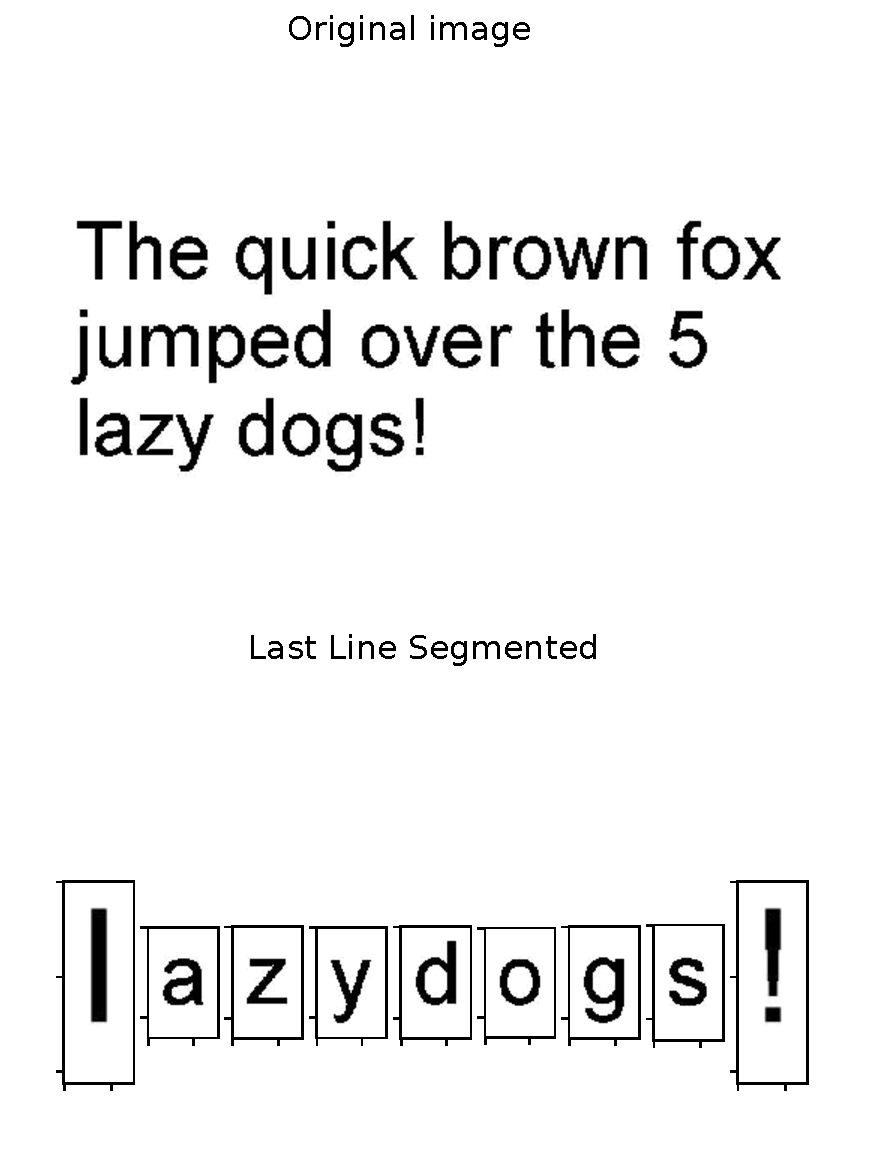
\includegraphics[width=5 cm]{images/sample3segmented.pdf}}
\caption{Applying segmentation}
\label{fig:segment}
\end{figure}

\section{Application}

OCR converts images to machine-readable text. That will make it the
initial tool that needs to be used for processing any documents or
simply any written material in a digital image, which has been
captured by a camera \cite{www-ocr-wiki}. It’s output can be stored significantly more
compact than scanned images. But beyond that, it enables us to process
the output information for numerous applications. Examples of these
applications include creating a narrator machine to help the visually
impaired read nondigital documents and signs, or automatic recognition
of automobile number plates.


\section{License}
The project is developed under the open source Apache License 2.0. The license
file is included in the Git repository of the project.
The packages and softwares used in developing the project include OpenCV,
Python 2.7, Ansible, Cloudmesh. All of these packages are open-source. 
The license file for OpenCV is included in the project repository
(CV\_LICENSE.txt).


\section{Cloud Deployment} 

Automatic deployment of program on virtual environment was done using
Ansible \cite{www-ansible} .The jobs were collected, organized in 
Playbooks \cite{www-ansible-playbook} and run on virtual clusters provided
by Chameleon Cloud \cite{www-chameleoncloud}.
The tasks include Installing the essential libraries on the remote machine
and running the program.
The VM reservations were done using Cloudmesh Client. Three Ansible playbooks are used, one for 
deploying the software stack, one for running the OCR codes on a standard dataset
and another one for running it on an arbitrary image. The software stack
required for running the program includes the following components:
\begin{enumerate}
\item {\bfseries Git} The Git module is needed for cloning the OCR Python codes. 
It is installed using apt module.
\item{\bfseries OpenCV} OpenCV, as discussed in the previous sections, has become 
the standard library of computer vision. It is used in this project for multiple 
purposes. As this library is extensive, its installation may take a significant time.
Hence, we tried to examine all the possible ways to install it. Building from the source,
which is the recommended way for installing it (and any other package) took more than
20 minutes. Even after that, connecting it to the existing Python installation on the
VMs was problematic. The alternative ways include using PyPi, Conda (Anaconda package
management system), and apt. After trial and error, Apt appeared to be the best solution
with installation time of less than 5 minutes and hassle-free python integration. It can 
be easily installed on VMs using Ansible apt module. So we chose this method.
\item {\bfseries OCR Code} The codes of the program were checked in the project
repository. An Ansible role cloned these codes into each node of the cluster.
\item{\bfseries Dataset} An Ansible role was used to download and extract the
dataset. Unarchive module was used for this purpose.
\end{enumerate}


\section{Dataset}
The dataset used in our project for training the KNN is Chars74k \cite{chars74k-dataset}.
This dataset provides an extensive collection of English letters and digits, 
in handwritten form or in various computer fonts \cite{de2009character}. In this project, a subset 
of the data, including characters from computer fonts with 4 variations (combinations
of italic, bold and normal) was used. The glyphs in this subset include 0-9, A-Z, and a-z.
For each glyph, there are 1016 different files, each with one font. However, some of the fonts
are similar to each other.
\newline
Before this dataset, the MNIST handwritten digits database were used for preliminary 
purposes \cite{mnist-dataset}.

\section{Benchmarking}

After wrapping all the necessary material, the code was run in a role and the result
was saved in text files, using another role. The accuracy of classification is printed
in the console of the local machine.
The program was first deployed on single VMs that were reserved manually using 
Cloudmesh Client. Later on, clusters of 2-4 nodes were used to measure the execution
time of deployment. Note that for running the benchmark, there is a trade-off between the runtime
and accuracy of classification. The more samples are used for training the dataset, the higher the
accuracy will be achieved and of course the longer execution time is needed. 

\subsection{Sample size analysis}

Running a dataset of 50 images as the test and train data
with K=5, takes around 20 seconds and yieds an accuracy of 65\%. The time complexity
of the algorithm is O(n2), thus, using 100 samples will multiply the runtime by 4. 
However, as the dataset used contains 74k images, there is still significant diversity
among 100 images. As a result, using 100 images only improves the classification 
accuracy up to 75\%. Changing the number of nodes does not affect the runtime, unless paralellization
is exploited.

Each VM on Chameleon Cloud has only 1 core, 2050076 kB (2 GB) of RAM, and 20 GB of storage.
Due to small size of RAM, we had to keep the number of training samples under 200.

\subsection{Cluster size analysis}

In this section, the sample size is around 50 different fonts for training the classifier and another 50 for testing it.

For the cluster of \textbf{2 nodes}:
It took 67 seconds to deploy (allocate) the cluster, 153 seconds to install the software stack
and dataset on the nodes, and 169 seconds to run the benchmark on them. The accuracy of classification on one of the nodes was 72.23 and on the other, it was 70.84.

For the cluster of \textbf{3 nodes}:
It took 98 seconds to deploy (allocate) the cluster, 170 seconds to install the stack and
180 seconds to run the benchmark.

For the cluster of \textbf{4 nodes}:
It took 131 seconds to deploy (allocate) the cluster, 175 seconds to install the stack and
187 seconds to run the benchmark.
As we can see, the higher number of nodes will only add to the time of cluster creation. As the nodes are
quite similar, the execution time of the tasks which run in parallel is similar.

\subsection{OCR on arbitrary images}
As the arbitrary images can be significantly different from 
the standard dataset, the sample size needs to be much higher. However, due to small size of RAM, for running OCR on arbitrary images, we only used a sample size of 200. That causes the accuracy of OCR to be very low, around 20\%.


\begin{figure}[H]
\centering
\fbox{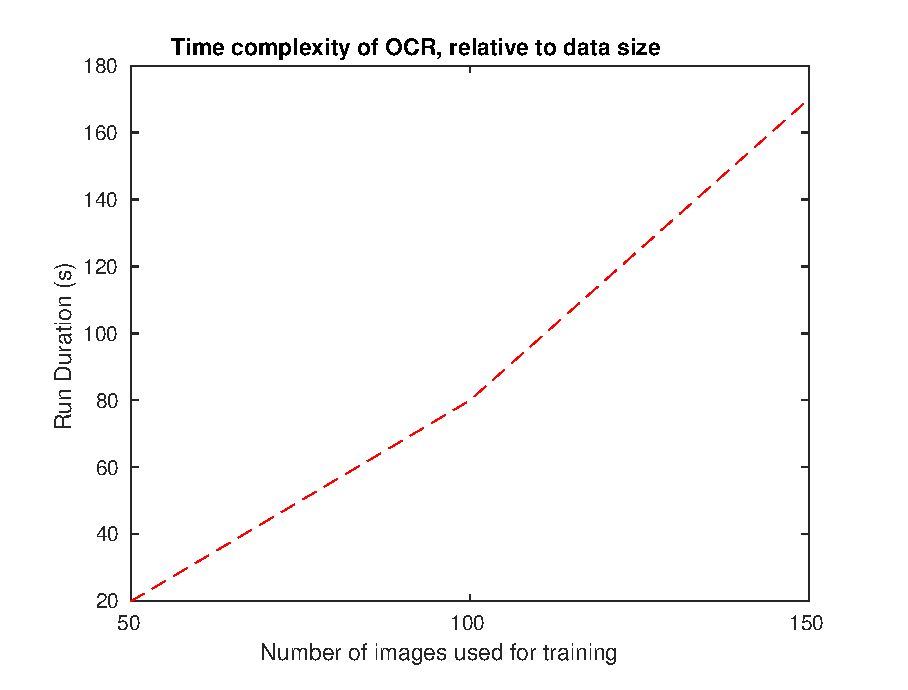
\includegraphics[width=8 cm]{images/time_complexity.eps}}
\caption{Time complexity of running OCR on Chameleon Cloud}
\end{figure}

\section{Reproducibility}
Instructions on reproduction of the project are provided in the project 
repository \cite{git-self-code}.


\section{Future Work}
For improving the current OCR system, various kinds of sophisticated structural features
can be added to feature extraction. It can also be extended to operate on languages other
than English. In order to improve the performance, the power of multiple cores/VMs can be
used for parallelization, so that after segmentation, each VM will operate on one line
of the text. Thus, multiple lines can be processed at the same time. For improving the
recognition accuracy, a lexicon can be used to evaluate the validity of the words that
have been formed by OCR, and then possibly correct them to the closest word in the lexicon.


\section{ACKNOWLEDGEMENT}
A very special thanks to Professor Gregor von Laszewski and the
teaching assistants Miao Zhang and Dimitar Nikolov for all the support
and guidance. This project proposal is written during the spring 2017
semester course {I524: Big Data and Open Source Software Projects} at
Indiana University Bloomington.

\section*{AUTHOR BIOGRAPHIES}
\begingroup
\setlength\intextsep{0pt}
\begin{minipage}[t][3.2cm][t]{1.0\columnwidth} % Adjust height [3.2cm] as required for separation of bio photos.
  \begin{wrapfigure}{L}{0.25\columnwidth}
    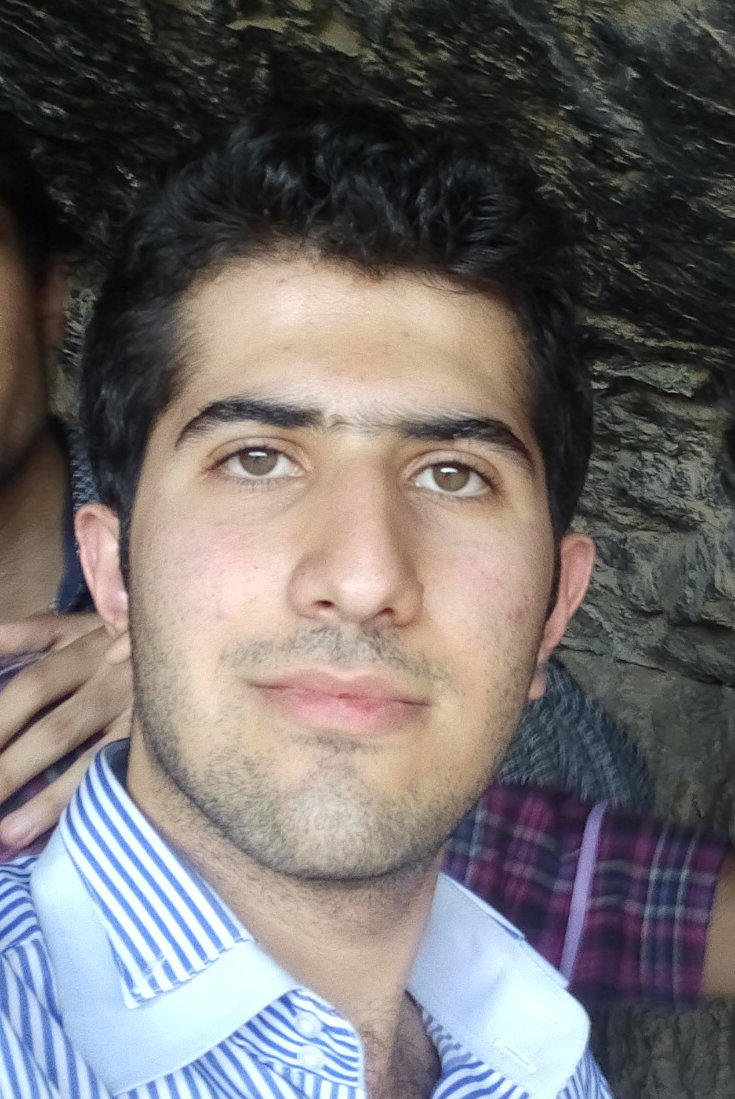
\includegraphics[width=0.25\columnwidth]{images/saber.jpg}
  \end{wrapfigure}
  \noindent
  {\bfseries Saber Sheybani} received his B.S. (Electrical Engineering - 
  Minor in Control Engineering) from University of Tehran.  He is currently 
  a PhD student of Intelligent Systems Engineering - Neuroengineering at 
  Indiana University Bloomington.
\end{minipage}
\begin{minipage}[t][3.2cm][t]{1.0\columnwidth} % Adjust height [3.2cm] as required for separation of bio photos.
  \begin{wrapfigure}{L}{0.25\columnwidth}
    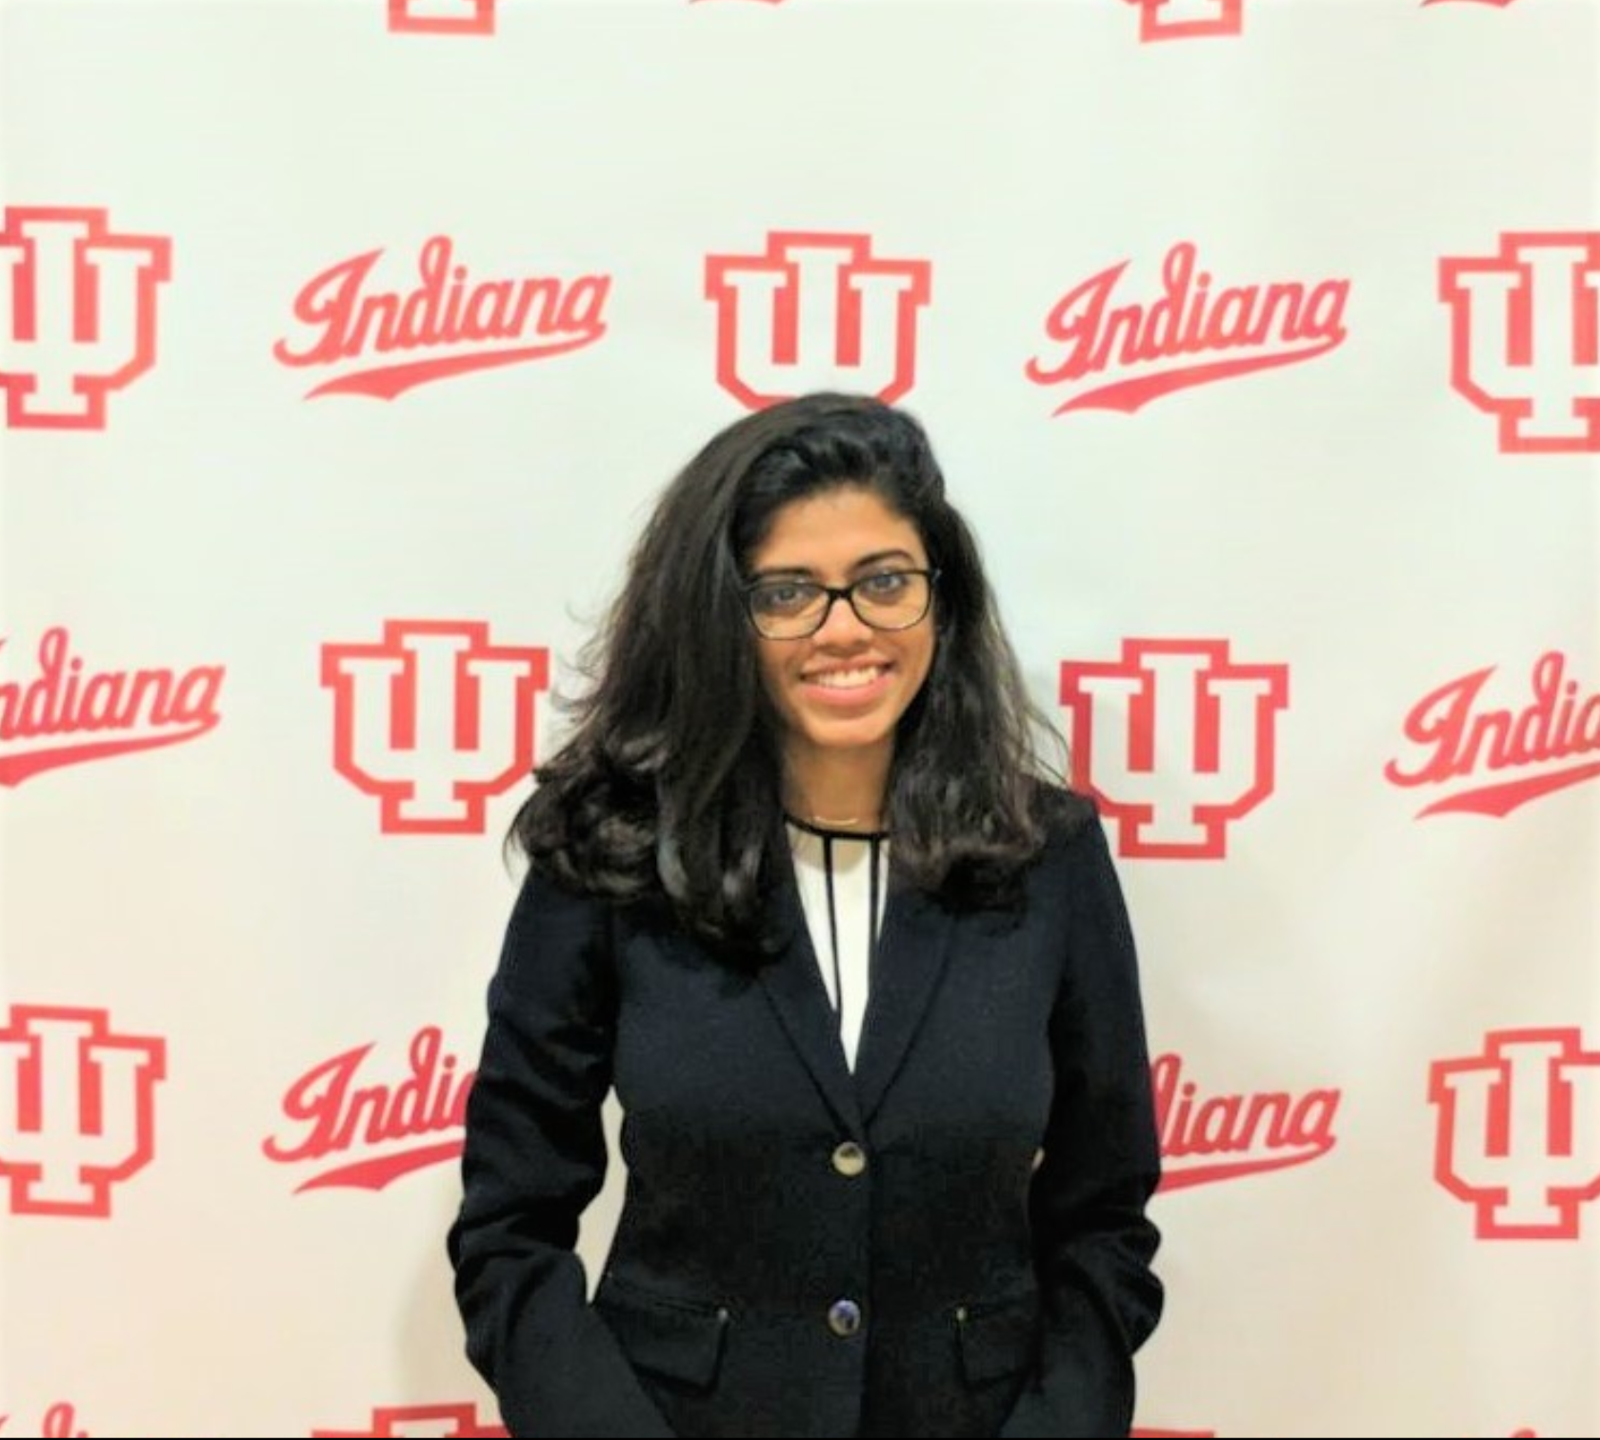
\includegraphics[width=0.25\columnwidth]{images/sushmita.png}
  \end{wrapfigure}
  \noindent
  {\bfseries Sushmita Sivaprasad} is a graduate student in Data Science at
Indiana University under the department of Informatics and
Computing. She had completed her bachelors in Electronics and
Communication from SRM University , India and her master's in
International Business from Hult International Business School, UAE.

\end{minipage}
\endgroup

\section{WORK BREAKDOWN}

The following was the work distribution followed for the project,
\begin{itemize}
\item {\bfseries Sushmita Sivaprasad} : Researched on the background of implementing
the ocr technology, briefed on the system configurations and the
technologies that can be used. She implemented the preprocessing steps
to remove the noise and inaccuracies in the image file before
implementing the K means algorithm. Contributed to the writing of the
report.
\item {\bfseries Saber Sheybani} : Implemented the cloud deployment on
chameleon cloud and has done the benchmarking of the on the chameleon
cloud. Contributed to the writing of the report.
\end{itemize}

\bibliography{references}

\end{document}
